\documentclass[conference]{IEEEtran}
\usepackage{graphicx}
\begin{document}
\title{Project BlackJack}
\author{
\IEEEauthorblockN{Jelle Biebaut, Daan Delva, Jari Meire, Niels Wauters}
\IEEEauthorblockA{HoGent\\Onderzoekstechnieken\\Groep16}}
\maketitle

\IEEEpeerreviewmaketitle

\section{Inleiding}
In het kader van het opleidingsonderdeel Onderzoekstechnieken kregen we de opdracht om onderzoek te voeren naar blackjack. Blackjack is een {\it card game} met eenvoudige spelregels. Een speler probeert een score te behalen zo dicht mogelijk bij 21 zonder dat hij erboven gaat, hetzelfde geldt voor de dealer. Zolang dat geen van beide boven de 21 gaat, wint de hoogste score. Als beide spelers een gelijke score hebben, wint de dealer.
Maar achter dit spel zijn verschillende strategie\"en bedacht om zo veel mogelijk te kunnen winnen. De bedoeling van dit onderzoek is om een zo goed mogelijke strategie te vinden voor het spelen van dit spelletje. We maken hiervoor gebruik van simulatie-software om tot onze resultaten te komen.\\*
 
\hfill April 20, 2015

\subsection{Onderzoeksvraag}
\textbf{Welke strategie geeft je het meeste kans op een positieve winst ?}\\*
Dit gaan we nagaan door onze beste eigen strategie naast een aantal bestaande strategie\"en te leggen.
Daarna te vergelijken via onze simulatie software wanneer we de grootste kans hebben op een positieve winst. Daaruit hopen we een goed resultaat te halen dat ons zal helpen bij het bepalen van de beste strategie.

\subsection{Deelonderzoeksvraag} 
\textbf{Welke opties geven je het meeste kans op een positieve winst ?} 
\footnote{ Deze opties zijn {\it dealer stand of hit op een soft 17}, {\it verdubbelen van inzet bij elk paar of enkel bij 9, 10 of 11},
    {\it verdubbelen van inzet na elke split is toegestaan of niet} en {\it surrenderen of niet}}\\*
We gaan na welke van deze opties de meest effici\"entste combinatie is en waarbij we dus de meeste kans hebben op een positieve winst.
We onderzoeken eerst alle strategie\"en met onze eerste 3 opties (dealer stand of hit op een soft 17, verdubbelen van inzet bij elk paar of enkel bij 9, 10 of 11 en verdubbelen van inzet na elke split is toegestaan of niet). Daarna kiezen we de beste 4 strategie\"en en passen we onze laatste optie daar op toe om zo tot onze eigen beste strategie te komen. \\*
We zorgen ervoor dat onze inzet nooit veranderd, onze standaard inzet is steeds 1\$, via onze simulatie software krijgen we steeds een \textit{average profit}, \textit{house edge}, de kans op een winst groter dan 5\$ en een verlies groter dan 5\$. 

\newpage

\section{Strategie\"en}
We gaan eerst onderzoeken welke van onze opties het beste resultaat geeft. Bij elk van onze opties hebben we een \textit{basic strategy}
opgesteld en deze in onze simulator gestoken. Dus strategie 1 is de combinatie van dealer stands op een soft 17, we verdubbelen alle paren en
verdubbeling na een split is niet toegestaan. Strategie 2 is de combinatie van dealer stands op een soft 17, we verdubbelen alle paren en
verdubbeling na een split is toegestaan. En zo gaan we verder tot we in elke strategie een andere combinatie hebben van onze opties.\\*
Hierna gaan we alle strategie\"en vergelijken met elkaar en halen we er de 4 beste uit en daar passen we onze laatste optie op toe, \textit{surrender}. Onze simulatie doen we steeds met 6 decks en de speler mag split doen tot een maximum van 4 handen.

\subsection{Welke van onze eigen strategie is de beste ? (Deel 1)}
In deze paragraaf gaan we onze beste 4 strategie\"en bespreken zonder de surrender, daarna bespreken we de beste 2 strategie\"en met surrender.\\*


\paragraph{Strategie 1}
% Dit is onze strategie 2 in het document "Soorten strategie\"en"

Deze strategie bestaat uit de combinatie van dealer stands op een soft 17, we verdubbelen de inzet bij alle paren en verdubbeling van de inzet na een split is toegestaan. \footnote{ Bij bovenstaande tabel betekenen volgende letters dit: S staat voor player Stand, H staat voor player Hit, D staat voor Double en Hit als double toegestaan is, DS staat voor Double en Stand als double niet toegestaan is en P staat voor Split. Hetzelfde geldt voor de andere tabellen.}
Dan bekomen we deze \textit{basic strategy} :

\begin{table}[ht]
\tiny
\centering
\begin{tabular}{|l|l|l|l|l|l|l|l|l|l|l|}
\hline

{Player hand} & \multicolumn{10}{c|}{Dealer's face-up card}     \\ \cline{2-11} 
                             & 2 & 3 & 4 & 5 & 6 & 7 & 8 & 9 & 10 & A \\ \hline
\multicolumn{11}{|c|}{\textbf{Hard totals}}                           \\ \hline
17-20       								 & S & S & S & S & S & S & S & S & S & S  \\ \hline
16                           & S & S & S & S & S & H & H & H & H & H  \\ \hline
15                           & S & S & S & S & S & H & H & H & H & H  \\ \hline
13-14                        & S & S & S & S & S & H & H & H & H & H  \\ \hline
12                           & H & H & S & S & S & H & H & H & H & H  \\ \hline
11                           & D & D & D & D & D & D & D & D & D & H  \\ \hline
10                           & D & D & D & D & D & D & D & D & H & H  \\ \hline
9                            & H & D & D & D & D & H & H & H & H & H  \\ \hline
5-8                          & H & H & H & H & H & H & H & H & H & H  \\ \hline

\multicolumn{11}{|c|}{\textbf{Soft totals}}                           \\ \hline
                             & 2 & 3 & 4 & 5 & 6 & 7 & 8 & 9 & 10 & A \\ \hline
A,8-A,9                      & S & S & S & S & S & S & S & S & S & S  \\ \hline
A,7                          & S & DS & DS & DS & DS & S & S & H & H & H  \\ \hline
A,6                          & H & D & D & D & D & H & H & H & H & H  \\ \hline
A,4-A,5                      & H & H & D & D & D & H & H & H & H & H  \\ \hline
A,2-A,3                      & H & H & H & D & D & H & H & H & H & H  \\ \hline

\multicolumn{11}{|c|}{\textbf{Pairs}}                                 \\ \hline
                             & 2 & 3 & 4 & 5 & 6 & 7 & 8 & 9 & 10 & A \\ \hline
A,A                          & P & P & P & P & P & P & P & P & P & P  \\ \hline
10,10                        & S & S & S & S & S & S & S & S & S & S  \\ \hline
9,9                          & P & P & P & P & P & S & P & P & S & S  \\ \hline
8,8                          & P & P & P & P & P & P & P & P & P & P  \\ \hline
7,7                          & P & P & P & P & P & P & H & H & H & H  \\ \hline
6,6                          & H & P & P & P & P & H & H & H & H & H  \\ \hline
5,5                          & D & D & D & D & D & D & D & D & H & H  \\ \hline
4,4                          & H & H & H & H & H & H & H & H & H & H  \\ \hline
2,2-3,3                      & H & H & P & P & P & P & H & H & H & H  \\ \hline
\end{tabular}
\end{table}


\paragraph{Strategie 2}
% Dit is onze strategie 3 in het document "Soorten strategie\"en"

Deze strategie bestaat uit de combinatie van dealer stands op een soft 17, we verdubbelen de inzet alleen bij de paren 9, 10 en 11 en verdubbeling van de inzet na een split is toegestaan.\\*
Dan bekomen we deze \textit{basic strategy} :

\begin{table}[ht]
\tiny
\centering
\begin{tabular}{|l|l|l|l|l|l|l|l|l|l|l|}
\hline

{Player hand} & \multicolumn{10}{c|}{Dealer's face-up card}     \\ \cline{2-11} 
                             & 2 & 3 & 4 & 5 & 6 & 7 & 8 & 9 & 10 & A \\ \hline
\multicolumn{11}{|c|}{\textbf{Hard totals}}                           \\ \hline
17-20       								 & S & S & S & S & S & S & S & S & S & S  \\ \hline
16                           & S & S & S & S & S & H & H & H & H & H  \\ \hline
15                           & S & S & S & S & S & H & H & H & H & H  \\ \hline
13-14                        & S & S & S & S & S & H & H & H & H & H  \\ \hline
12                           & H & H & S & S & S & H & H & H & H & H  \\ \hline
11                           & D & D & D & D & D & D & D & D & D & H  \\ \hline
10                           & D & D & D & D & D & D & D & D & H & H  \\ \hline
9                            & H & D & D & D & D & H & H & H & H & H  \\ \hline
5-8                          & H & H & H & H & H & H & H & H & H & H  \\ \hline

\multicolumn{11}{|c|}{\textbf{Soft totals}}                           \\ \hline
                             & 2 & 3 & 4 & 5 & 6 & 7 & 8 & 9 & 10 & A \\ \hline
A,8-A,9                      & S & S & S & S & S & S & S & S & S & S  \\ \hline
A,7                          & S & S & S & S & S & S & S & H & H & H  \\ \hline
A,6                          & H & H & H & H & H & H & H & H & H & H  \\ \hline
A,4-A,5                      & H & H & H & H & H & H & H & H & H & H  \\ \hline
A,2-A,3                      & H & H & H & H & H & H & H & H & H & H  \\ \hline

\multicolumn{11}{|c|}{\textbf{Pairs}}                                 \\ \hline
                             & 2 & 3 & 4 & 5 & 6 & 7 & 8 & 9 & 10 & A \\ \hline
A,A                          & P & P & P & P & P & P & P & P & P & P  \\ \hline
10,10                        & S & S & S & S & S & S & S & S & S & S  \\ \hline
9,9                          & P & P & P & P & P & S & P & P & S & S  \\ \hline
8,8                          & P & P & P & P & P & P & P & P & P & P  \\ \hline
7,7                          & P & P & P & P & P & P & H & H & H & H  \\ \hline
6,6                          & P & P & P & P & P & H & H & H & H & H  \\ \hline
5,5                          & D & D & D & D & D & D & D & D & H & H  \\ \hline
4,4                          & H & H & H & P & P & H & H & H & H & H  \\ \hline
2,2-3,3                      & P & P & P & P & P & P & H & H & H & H  \\ \hline
\end{tabular}
\end{table}



\paragraph{Strategie 3}
% Dit is onze strategie 7 in het document "Soorten strategie\"en"

Deze strategie bestaat uit de combinatie van dealer hits op een soft 17, we verdubbelen de inzet bij alle paren en verdubbeling van inzet na een split is toegestaan.\\*
Dan bekomen we deze \textit{basic strategy} :

\begin{table}[ht]
\tiny
\centering
\begin{tabular}{|l|l|l|l|l|l|l|l|l|l|l|}
\hline

{Player hand} & \multicolumn{10}{c|}{Dealer's face-up card}     \\ \cline{2-11} 
                             & 2 & 3 & 4 & 5 & 6 & 7 & 8 & 9 & 10 & A \\ \hline
\multicolumn{11}{|c|}{\textbf{Hard totals}}                           \\ \hline
17-20       								 & S & S & S & S & S & S & S & S & S & S  \\ \hline
16                           & S & S & S & S & S & H & H & H & H & H  \\ \hline
15                           & S & S & S & S & S & H & H & H & H & H  \\ \hline
13-14                        & S & S & S & S & S & H & H & H & H & H  \\ \hline
12                           & H & H & S & S & S & H & H & H & H & H  \\ \hline
11                           & D & D & D & D & D & D & D & D & D & D  \\ \hline
10                           & D & D & D & D & D & D & D & D & H & H  \\ \hline
9                            & H & D & D & D & D & H & H & H & H & H  \\ \hline
5-8                          & H & H & H & H & H & H & H & H & H & H  \\ \hline

\multicolumn{11}{|c|}{\textbf{Soft totals}}                           \\ \hline
                             & 2 & 3 & 4 & 5 & 6 & 7 & 8 & 9 & 10 & A \\ \hline
A,8-A,9                      & S & S & S & S & DS & S & S & S & S & S  \\ \hline
A,7                          & DS & DS & DS & DS & DS & S & S & H & H & H  \\ \hline
A,6                          & H & D & D & D & D & H & H & H & H & H  \\ \hline
A,4-A,5                      & H & H & D & D & D & H & H & H & H & H  \\ \hline
A,2-A,3                      & H & H & H & D & D & H & H & H & H & H  \\ \hline

\multicolumn{11}{|c|}{\textbf{Pairs}}                                 \\ \hline
                             & 2 & 3 & 4 & 5 & 6 & 7 & 8 & 9 & 10 & A \\ \hline
A,A                          & P & P & P & P & P & P & P & P & P & P  \\ \hline
10,10                        & S & S & S & S & S & S & S & S & S & S  \\ \hline
9,9                          & P & P & P & P & P & S & P & P & S & S  \\ \hline
8,8                          & P & P & P & P & P & P & P & P & P & P  \\ \hline
7,7                          & P & P & P & P & P & P & H & H & H & H  \\ \hline
6,6                          & P & P & P & P & P & H & H & H & H & H  \\ \hline
5,5                          & D & D & D & D & D & D & D & D & H & H  \\ \hline
4,4                          & H & H & H & H & H & H & H & H & H & H  \\ \hline
2,2-3,3                      & P & P & P & P & P & P & H & H & H & H  \\ \hline
\end{tabular}
\end{table}

\newpage

\paragraph{Strategie 4}
% Dit is onze strategie 9 in het document "Soorten strategie\"en"

Deze strategie bestaat uit de combinatie van dealer hits op een soft 17, we verdubbelen de inzet alleen bij de paren 9, 10 en 11 en verdubbeling na een split is toegestaan.\\*
Dan bekomen we deze \textit{basic strategy} :

\begin{table}[ht]
\tiny
\centering
\begin{tabular}{|l|l|l|l|l|l|l|l|l|l|l|}
\hline

{Player hand} & \multicolumn{10}{c|}{Dealer's face-up card}     \\ \cline{2-11} 
                             & 2 & 3 & 4 & 5 & 6 & 7 & 8 & 9 & 10 & A \\ \hline
\multicolumn{11}{|c|}{\textbf{Hard totals}}                           \\ \hline
17-20       								 & S & S & S & S & S & S & S & S & S & S  \\ \hline
16                           & S & S & S & S & S & H & H & H & H & H  \\ \hline
15                           & S & S & S & S & S & H & H & H & H & H  \\ \hline
13-14                        & S & S & S & S & S & H & H & H & H & H  \\ \hline
12                           & H & H & S & S & S & H & H & H & H & H  \\ \hline
11                           & D & D & D & D & D & D & D & D & D & H  \\ \hline
10                           & D & D & D & D & D & D & D & D & H & H  \\ \hline
9                            & H & D & D & D & D & H & H & H & H & H  \\ \hline
5-8                          & H & H & H & H & H & H & H & H & H & H  \\ \hline

\multicolumn{11}{|c|}{\textbf{Soft totals}}                           \\ \hline
                             & 2 & 3 & 4 & 5 & 6 & 7 & 8 & 9 & 10 & A \\ \hline
A,8-A,9                      & S & S & S & S & S & S & S & S & S & S  \\ \hline
A,7                          & S & S & S & S & S & S & S & H & H & H  \\ \hline
A,6                          & H & H & H & H & H & H & H & H & H & H  \\ \hline
A,4-A,5                      & H & H & H & H & H & H & H & H & H & H  \\ \hline
A,2-A,3                      & H & H & H & H & H & H & H & H & H & H  \\ \hline

\multicolumn{11}{|c|}{\textbf{Pairs}}                                 \\ \hline
                             & 2 & 3 & 4 & 5 & 6 & 7 & 8 & 9 & 10 & A \\ \hline
A,A                          & P & P & P & P & P & P & P & P & P & P  \\ \hline
10,10                        & S & S & S & S & S & S & S & S & S & S  \\ \hline
9,9                          & P & P & P & P & P & S & P & P & S & S  \\ \hline
8,8                          & P & P & P & P & P & P & P & P & P & P  \\ \hline
7,7                          & P & P & P & P & P & P & H & H & H & H  \\ \hline
6,6                          & P & P & P & P & P & H & H & H & H & H  \\ \hline
5,5                          & D & D & D & D & D & D & D & D & H & H  \\ \hline
4,4                          & H & H & H & P & P & H & H & H & H & H  \\ \hline
2,2-3,3                      & P & P & P & P & P & P & H & H & H & H  \\ \hline
\end{tabular}
\end{table}

\paragraph{De beste strategie}

Uit onze resultaten na het simuleren van al onze strategie\"en zijn bovenstaande 5 er het beste uitgekomen. En dus opteren we ervoor om deze 5 te vergelijken met elkaar. \\*

Strategie 1 heeft een average profit van -0,29 en een house edge van 0,29. Daarbij hebben we een kans van bijna 32\% dat onze winst groter is dan 5\$ en een kans van 34\% dat we een verlies leiden van groter dan 5\$. \\*

Strategie 2 heeft een average profit van -0,46 en een house edge van 0,46. Daarbij hebben we een kans van 31,21\% dat onze winst groter is dan 5\$ en een kans van 34\% dat we een verlies leiden van groter dan 5\$.\\*

Strategie 3 heeft een average profit van -0,87 en een house edge van 0,87. Daarbij hebben we een kans van 30,85\% dat onze winst groter is dan 5\$ en een kans van bijna 36\% dat we een verlies leiden van groter dan 5\$.\\*

Strategie 4 heeft een average profit van -0,78 en een house edge van 0,78. Daarbij hebben we een kans van bijna 30,5\% dat onze winst groter is dan 5\$ en een kans van 35,57\% dat we een verlies leiden van groter dan 5\$. \\*
 
Zo zien we dat dus onze eerste strategie ons het dichtst brengt bij een positieve winst. We weten dat we nooit een positieve winst zouden kunnen halen aangezien iedereen dan die strategie zou toepassen en casino's dan veel verlies zouden lijden.
We hebben nu wel 1 optie die nog steeds niet gebruikt is, de optie surrender. Aangezien je in de realiteit ook de mogelijkheid hebt om te surrenderen, hebben we nu van deze 4 vorige strategie\"en 4 nieuwe strategie\"en gemaakt met de optie om te surrenderen. 
 
 
\newpage

\subsection{Welke van onze eigen strategie is het beste ? (Deel 2)}
In deze paragraaf onderzoeken we welke van bovenstaande strategieën het beste is met surrender.\\*

\paragraph{Strategie 1 met surrender}
% Dit is onze strategie 5 in het document "Soorten strategie\"en"

Deze strategie bestaat uit de combinatie van dealer stands op een soft 17, we verdubbelen de inzet bij alle paren en verdubbeling van de inzet na een split is toegestaan. \footnote{ Bij bovenstaande tabel betekenen volgende letters dit: RH staat voor Surrender en Hit als surrender niet is toegestaan, RS staat voor Surrender en Stand als surrender niet is toegestaan en RP staat voor Surrender en Split als surrender niet is toegestaan}
Dan bekomen we deze \textit{basic strategy} :

\begin{table}[ht]
\tiny
\centering
\begin{tabular}{|l|l|l|l|l|l|l|l|l|l|l|}
\hline

{Player hand} & \multicolumn{10}{c|}{Dealer's face-up card}     \\ \cline{2-11} 
                             & 2 & 3 & 4 & 5 & 6 & 7 & 8 & 9 & 10 & A \\ \hline
\multicolumn{11}{|c|}{\textbf{Hard totals}}                           \\ \hline
17-20       								 & S & S & S & S & S & S & S & S & S & S  \\ \hline
16                           & S & S & S & S & S & H & H & RH & RS & RH  \\ \hline
15                           & S & S & S & S & S & H & H & H & RH & H  \\ \hline
13-14                        & S & S & S & S & S & H & H & H & H & H  \\ \hline
12                           & H & H & S & S & S & H & H & H & H & H  \\ \hline
11                           & D & D & D & D & D & D & D & D & D & H  \\ \hline
10                           & D & D & D & D & D & D & D & D & H & H  \\ \hline
9                            & H & D & D & D & D & H & H & H & H & H  \\ \hline
5-8                          & H & H & H & H & H & H & H & H & H & H  \\ \hline

\multicolumn{11}{|c|}{\textbf{Soft totals}}                           \\ \hline
                             & 2 & 3 & 4 & 5 & 6 & 7 & 8 & 9 & 10 & A \\ \hline
A,8-A,9                      & S & S & S & S & S & S & S & S & S & S  \\ \hline
A,7                          & S & DS & DS & DS & DS & S & S & H & H & H  \\ \hline
A,6                          & H & D & D & D & D & H & H & H & H & H  \\ \hline
A,4-A,5                      & H & H & D & D & D & H & H & H & H & H  \\ \hline
A,2-A,3                      & H & H & H & D & D & H & H & H & H & H  \\ \hline

\multicolumn{11}{|c|}{\textbf{Pairs}}                                 \\ \hline
                             & 2 & 3 & 4 & 5 & 6 & 7 & 8 & 9 & 10 & A \\ \hline
A,A                          & P & P & P & P & P & P & P & P & P & P  \\ \hline
10,10                        & S & S & S & S & S & S & S & S & S & S  \\ \hline
9,9                          & P & P & P & P & P & S & P & P & S & S  \\ \hline
8,8                          & P & P & P & P & P & P & P & P & P & P  \\ \hline
7,7                          & P & P & P & P & P & P & H & H & H & H  \\ \hline
6,6                          & H & P & P & P & P & H & H & H & H & H  \\ \hline
5,5                          & D & D & D & D & D & D & D & D & H & H  \\ \hline
4,4                          & H & H & H & H & H & H & H & H & H & H  \\ \hline
2,2-3,3                      & H & H & P & P & P & P & H & H & H & H  \\ \hline
\end{tabular}
\end{table}


\paragraph{Strategie 2 met surrender}
% Dit is onze strategie 6 in het document "Soorten strategie\"en"

Deze strategie bestaat uit de combinatie van dealer stands op een soft 17, we verdubbelen de inzet alleen bij de paren 9, 10 en 11 en verdubbeling van de inzet na een split is toegestaan.\\*
Dan bekomen we deze \textit{basic strategy} :

\begin{table}[ht]
\tiny
\centering
\begin{tabular}{|l|l|l|l|l|l|l|l|l|l|l|}
\hline

{Player hand} & \multicolumn{10}{c|}{Dealer's face-up card}     \\ \cline{2-11} 
                             & 2 & 3 & 4 & 5 & 6 & 7 & 8 & 9 & 10 & A \\ \hline
\multicolumn{11}{|c|}{\textbf{Hard totals}}                           \\ \hline
17-20       								 & S & S & S & S & S & S & S & S & S & S  \\ \hline
16                           & S & S & S & S & S & H & H & RH & RS & RH  \\ \hline
15                           & S & S & S & S & S & H & H & H & RH & H  \\ \hline
13-14                        & S & S & S & S & S & H & H & H & H & H  \\ \hline
12                           & H & H & S & S & S & H & H & H & H & H  \\ \hline
11                           & D & D & D & D & D & D & D & D & D & H  \\ \hline
10                           & D & D & D & D & D & D & D & D & H & H  \\ \hline
9                            & H & D & D & D & D & H & H & H & H & H  \\ \hline
5-8                          & H & H & H & H & H & H & H & H & H & H  \\ \hline

\multicolumn{11}{|c|}{\textbf{Soft totals}}                           \\ \hline
                             & 2 & 3 & 4 & 5 & 6 & 7 & 8 & 9 & 10 & A \\ \hline
A,8-A,9                      & S & S & S & S & S & S & S & S & S & S  \\ \hline
A,7                          & S & S & S & S & S & S & S & H & H & H  \\ \hline
A,6                          & H & H & H & H & H & H & H & H & H & H  \\ \hline
A,4-A,5                      & H & H & H & H & H & H & H & H & H & H  \\ \hline
A,2-A,3                      & H & H & H & H & H & H & H & H & H & H  \\ \hline

<<<<<<< HEAD
\begin{figure}
\centering
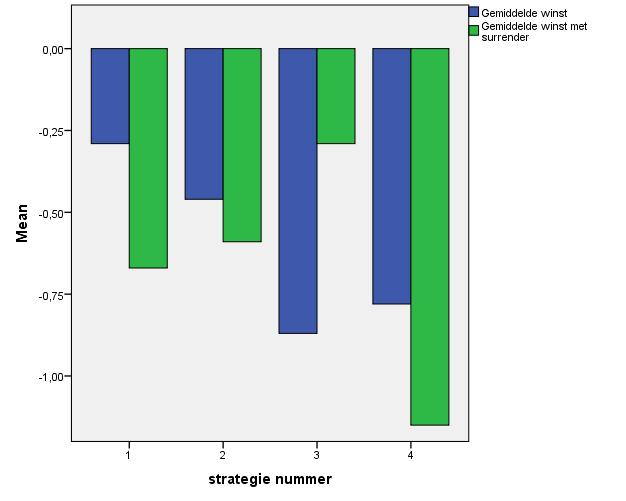
\includegraphics[width=0.7\linewidth]{OUTPUT1}
\caption{}
\label{fig:OUTPUT1}
\end{figure}



=======
\multicolumn{11}{|c|}{\textbf{Pairs}}                                 \\ \hline
                             & 2 & 3 & 4 & 5 & 6 & 7 & 8 & 9 & 10 & A \\ \hline
A,A                          & P & P & P & P & P & P & P & P & P & P  \\ \hline
10,10                        & S & S & S & S & S & S & S & S & S & S  \\ \hline
9,9                          & P & P & P & P & P & S & P & P & S & S  \\ \hline
8,8                          & P & P & P & P & P & P & P & P & P & P  \\ \hline
7,7                          & P & P & P & P & P & P & H & H & H & H  \\ \hline
6,6                          & P & P & P & P & P & H & H & H & H & H  \\ \hline
5,5                          & D & D & D & D & D & D & D & D & H & H  \\ \hline
4,4                          & H & H & H & P & P & H & H & H & H & H  \\ \hline
2,2-3,3                      & P & P & P & P & P & P & H & H & H & H  \\ \hline
\end{tabular}
\end{table}
>>>>>>> origin/master

\newpage

\paragraph{Strategie 3 met surrender}
% Dit is onze strategie 11 in het document "Soorten strategie\"en"

Deze strategie bestaat uit de combinatie van dealer hits op een soft 17, we verdubbelen de inzet bij alle paren en verdubbeling van inzet na en split is toegestaan.\\*
Dan bekomen we deze \textit{basic strategy} :

\begin{table}[ht]
\tiny
\centering
\begin{tabular}{|l|l|l|l|l|l|l|l|l|l|l|}
\hline

{Player hand} & \multicolumn{10}{c|}{Dealer's face-up card}     \\ \cline{2-11} 
                             & 2 & 3 & 4 & 5 & 6 & 7 & 8 & 9 & 10 & A \\ \hline
\multicolumn{11}{|c|}{\textbf{Hard totals}}                           \\ \hline
18-20       								 & S & S & S & S & S & S & S & S & S & S  \\ \hline
17                           & S & S & S & S & S & S & S & S & S & RS  \\ \hline
16                           & S & S & S & S & S & H & H & RH & RS & RH  \\ \hline
15                           & S & S & S & S & S & H & H & H & RH & RH  \\ \hline
13-14                        & S & S & S & S & S & H & H & H & H & H  \\ \hline
12                           & H & H & S & S & S & H & H & H & H & H  \\ \hline
11                           & D & D & D & D & D & D & D & D & D & H  \\ \hline
10                           & D & D & D & D & D & D & D & D & H & H  \\ \hline
9                            & H & D & D & D & D & H & H & H & H & H  \\ \hline
5-8                          & H & H & H & H & H & H & H & H & H & H  \\ \hline

\multicolumn{11}{|c|}{\textbf{Soft totals}}                           \\ \hline
                             & 2 & 3 & 4 & 5 & 6 & 7 & 8 & 9 & 10 & A \\ \hline
A,8-A,9                      & S & S & S & S & DS & S & S & S & S & S  \\ \hline
A,7                          & DS & DS & DS & DS & DS & S & S & H & H & H  \\ \hline
A,6                          & H & D & D & D & D & H & H & H & H & H  \\ \hline
A,4-A,5                      & H & H & D & D & D & H & H & H & H & H  \\ \hline
A,2-A,3                      & H & H & H & D & D & H & H & H & H & H  \\ \hline

\multicolumn{11}{|c|}{\textbf{Pairs}}                                 \\ \hline
                             & 2 & 3 & 4 & 5 & 6 & 7 & 8 & 9 & 10 & A \\ \hline
A,A                          & P & P & P & P & P & P & P & P & P & P  \\ \hline
10,10                        & S & S & S & S & S & S & S & S & S & S  \\ \hline
9,9                          & P & P & P & P & P & S & P & P & S & S  \\ \hline
8,8                          & P & P & P & P & P & P & P & P & P & RP  \\ \hline
7,7                          & P & P & P & P & P & P & H & H & H & H  \\ \hline
6,6                          & P & P & P & P & P & H & H & H & H & H  \\ \hline
5,5                          & D & D & D & D & D & D & D & D & H & H  \\ \hline
4,4                          & H & H & H & P & P & H & H & H & H & H  \\ \hline
2,2-3,3                      & P & P & P & P & P & P & H & H & H & H  \\ \hline
\end{tabular}
\end{table}


\paragraph{Strategie 4 met surrender}
% Dit is onze strategie 12 in het document "Soorten strategie\"en"

Deze strategie bestaat uit de combinatie van dealer hits op een soft 17, we verdubbelen de inzet alleen bij de paren 9, 10 en 11 en verdubbeling na een split is toegestaan.\\*
Dan bekomen we deze \textit{basic strategy} :

\begin{table}[ht]
\tiny
\centering
\begin{tabular}{|l|l|l|l|l|l|l|l|l|l|l|}
\hline

{Player hand} & \multicolumn{10}{c|}{Dealer's face-up card}     \\ \cline{2-11} 
                             & 2 & 3 & 4 & 5 & 6 & 7 & 8 & 9 & 10 & A \\ \hline
\multicolumn{11}{|c|}{\textbf{Hard totals}}                           \\ \hline
18-20       								 & S & S & S & S & S & S & S & S & S & S  \\ \hline
17                           & S & S & S & S & S & S & S & S & S & RS  \\ \hline
16                           & S & S & S & S & S & H & H & RH & RS & RH  \\ \hline
15                           & S & S & S & S & S & H & H & H & RH & RH  \\ \hline
13-14                        & S & S & S & S & S & H & H & H & H & H  \\ \hline
12                           & H & H & S & S & S & H & H & H & H & H  \\ \hline
11                           & D & D & D & D & D & D & D & D & D & H  \\ \hline
10                           & D & D & D & D & D & D & D & D & H & H  \\ \hline
9                            & H & D & D & D & D & H & H & H & H & H  \\ \hline
5-8                          & H & H & H & H & H & H & H & H & H & H  \\ \hline

\multicolumn{11}{|c|}{\textbf{Soft totals}}                           \\ \hline
                             & 2 & 3 & 4 & 5 & 6 & 7 & 8 & 9 & 10 & A \\ \hline
A,8-A,9                      & S & S & S & S & S & S & S & S & S & S  \\ \hline
A,7                          & S & S & S & S & S & S & S & H & H & H  \\ \hline
A,6                          & H & H & H & H & H & H & H & H & H & H  \\ \hline
A,4-A,5                      & H & H & H & H & H & H & H & H & H & H  \\ \hline
A,2-A,3                      & H & H & H & H & H & H & H & H & H & H  \\ \hline

\multicolumn{11}{|c|}{\textbf{Pairs}}                                 \\ \hline
                             & 2 & 3 & 4 & 5 & 6 & 7 & 8 & 9 & 10 & A \\ \hline
A,A                          & P & P & P & P & P & P & P & P & P & P  \\ \hline
10,10                        & S & S & S & S & S & S & S & S & S & S  \\ \hline
9,9                          & P & P & P & P & P & S & P & P & S & S  \\ \hline
8,8                          & P & P & P & P & P & P & P & P & P & RP  \\ \hline
7,7                          & P & P & P & P & P & P & H & H & H & H  \\ \hline
6,6                          & P & P & P & P & P & H & H & H & H & H  \\ \hline
5,5                          & D & D & D & D & D & D & D & D & H & H  \\ \hline
4,4                          & H & H & H & P & P & H & H & H & H & H  \\ \hline
2,2-3,3                      & P & P & P & P & P & P & H & H & H & H  \\ \hline
\end{tabular}
\end{table}


\paragraph{De 'beste' strategie}

Ook hier hebben we dus alle opties ingegeven in onze simulator en krijgen we dezelfde 4 variabelen waar we de strategie\"en mee vergelijken. \\*
 
Strategie 1 met surrender heeft een average profit van -0,67 en een house edge van 0,67. Daarbij hebben we een kans van bijna 31\% dat onze winst groter is dan 5\$ en een kans van bijna 35\% dat we een verlies leiden van groter dan 5\$. \\*
 
Strategie 2 met surrender heeft een average profit van -0,59 en een house edge van 0,59. Daarbij hebben we een kans van 30,5\% dat onze winst groter is dan 5\$ en een kans van bijna 34,5\% dat we een verlies leiden van groter dan 5\$. \\*
 
Strategie 3 met surrender heeft een average profit van -0,29 en een house edge van 0,29. Daarbij hebben we een kans van iets meer dan 32\% dat onze winst groter is dan 5\$ en een kans van 34\% dat we een verlies leiden van groter dan 5\$. \\*
 
Strategie 4 met surrender heeft een average profit van -1,15 en een house edge van 1,15. Daarbij hebben we een kans van iets meer dan 29\% dat onze winst groter is dan 5\$ en een kans van bijna 37\% dat we een verlies leiden van groter dan 5\$. \\*
 
Hieruit kunnen we dus concluderen dat strategie 3 met surrender de beste strategie is die we kunnen hebben. Zo zien we maar dat het veranderen van 1 variabele grote veranderingen kan teweeg brengen. Zo is strategie 1 niet meer de beste strategie met surrender terwijl die die wel was zonder. En terwijl strategie 3 ons het minste kans op winst gaf zonder surrender, hebben we die kans nu verkleind tot de best mogelijke strategie.\\*

Dit zijn lang niet alle mogelijke strategie\"en maar we hebben besloten om niet elke optie op te nemen in ons onderzoek. Zo konden we ook de optie nemen om de dealer te laten 'peaken' naar zijn eerste kaart.


\section{Varia}




\begin{thebibliography}{1}

\bibitem{IEEEhowto:kopka}
H.~Kopka and P.~W. Daly, \emph{A Guide to \LaTeX}, 3rd~ed.\hskip 1em plus
  0.5em minus 0.4em\relax Harlow, England: Addison-Wesley, 1999.

\end{thebibliography}




\end{document}